\begin{figure}[t]
    \centering
    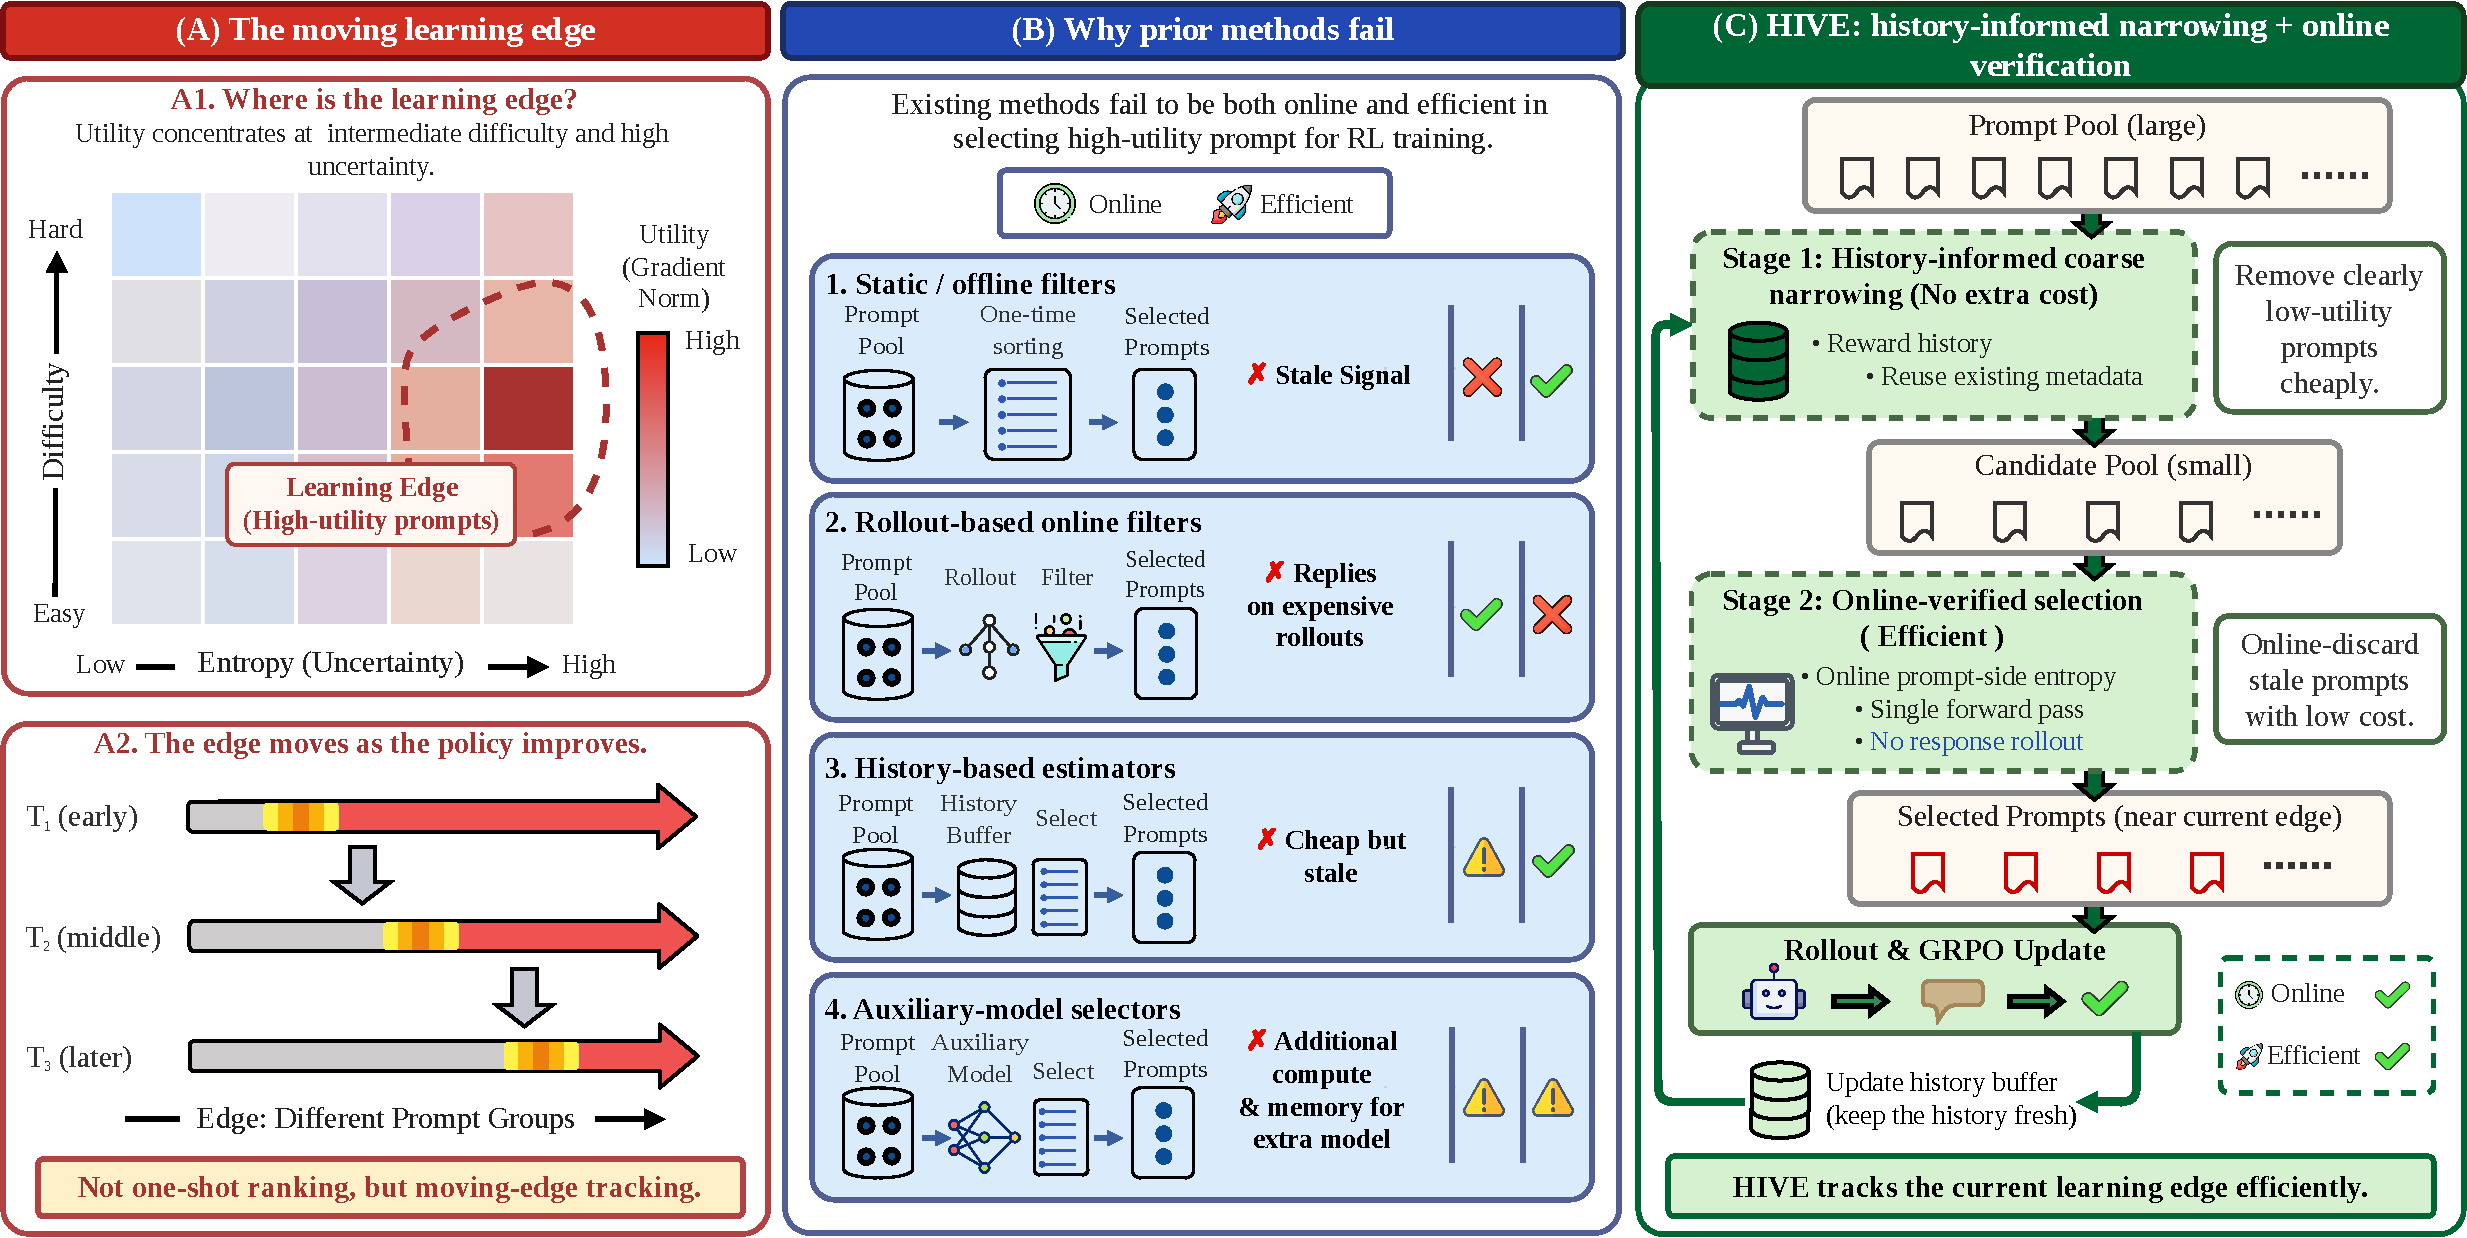
\includegraphics[width=0.98\linewidth]{figures/introduction/intro-fig-compare-motivate-1.pdf}
    \caption{\textbf{RLVR prompt selection is a moving-edge tracking problem.} (A) Utility concentrates at 
    intermediate difficulty and high uncertainty, and the learning edge is dynamic. 
    (B) Prior methods face limitations in efficiently selecting online high-utility prompts. (C) HIVE combines history-informed coarse narrowing with low-cost online 
    verification to track the current learning edge.}
    \label{fig:intro-compare-motivate}
    \vskip -0.2in
\end{figure}
% \red{1. re-write this caption 2.
%     delete precise. 3. redraw figure 3(d) to correspond to the A2 in figure 1. 4. shoud not be like curriculum, 
%     instead the utility of prompts across different step should be varying.}
